\section{Theory}
% Es sollen die wichtigsten theoretischen Formeln und Zusammenh�nge einmal ausf�hrlich erkl�rt werden
In this part elementary theoretical aspects for the experiment are discussed. The theory part is oriented by the scientific work of R. Gro� (cf. \cite{examenarbeit}) and the theory in the report of P. Pagel and J. Roggel (cf. \cite{philippundjensproto}).
\subsection{Spectroscopy of the ammoniak molekule}
It is possible to excite a molekule in differnt ways. Like atoms molekules can get to excited states by raising the energy eigenstate of an electron. Additionally the energy eingenstate of a molecule can be raised by changing the rotation energy with respect to the center of mass, also there are additional oszillation energyeigenstates of the atoms in the molecule. The energydifferences of these new eigenstates are not at the same frequency as it is measured in atoms. As a consequence it is possible to separate the effects and measure for example just energy differences of the frequeny spectrum from the rotation. The energy difference ist given by the sum of all energy differences (eq. \ref{eqn:Delta_E}).
\begin{align}
\Delta E = \Delta E_{electron} + \Delta E_{rot} + \Delta E_{osz}
\label{eqn:Delta_E}
\end{align}
The differences are typically in the range of Microwaves ($\Delta E_{rot} \sim$ \SI{e-3}{eV}) to visible light ($\Delta E_{electron} \sim$ \SI{10}{eV}), where the oscillation energy differences are at frequencys of infrared light (($\Delta E_{osz} \sim$ \SI{0,1}{eV})). In this experiment the rotation spectrum of the ammoniak molecule is intended to be measured. As shown in figure \ref{fig:ammoniak} the ammoniak mulecule possesses a tetraedic geometry.
\begin{figure}[H]
\centering
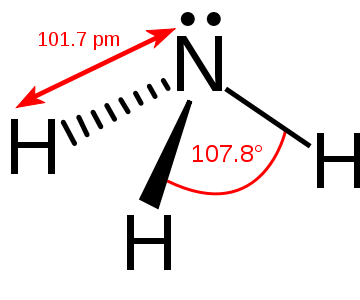
\includegraphics[clip = true, scale = 0.7]{Ammoniak.png}
\caption{The tetraedic geometrie of the ammoniak molecule. Source: \cite{ammoniak}}
\label{fig:ammoniak}
\end{figure}
The explanation of the energy quantisation is given by a quantum mechanical model, where the angular momentum and the z-component of the angular momentum are quantized. The quantum numbers that belong to these quantities are J (total angular momentum) and K (z-component). The relations between them are given by equation \ref{eqn:Quantum_numbers}.
\begin{align}
|\textbf{J}| = \hbar\cdot\sqrt{J(J+1)} \hspace{1cm} J_z = \hbar\cdot K
\label{eqn:Quantum_numbers}
\end{align}
The selection rules for the absorbtion lines of the ammoniak molecule are given by equation \ref{eqn:Auswahlregeln} (cf. \cite{examenarbeit}).
\begin{align}
\Delta J = +1 \hspace{1cm} \Delta K = 0
\label{eqn:Auswahlregeln}
\end{align}
\subsection{The inversion spectrum of ammoniak}
From the symmetry of the molecule, there are two possible positions for the nitrogen atom to be. This leads to a potential, which is shown in figure \ref{fig:inversion_potential}.
\begin{figure}[H]
\centering
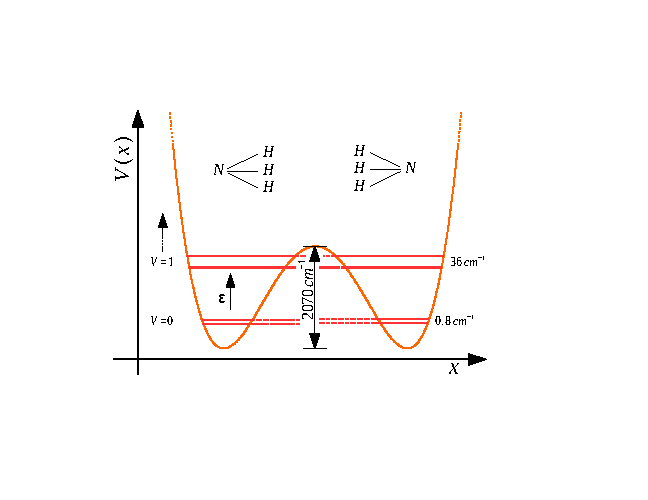
\includegraphics[clip = true, scale = 2]{Skizze2.pdf}
\caption{the inversion potential of tha ammoniak molecule. Source: \cite{philippundjensproto}}
\label{fig:inversion_potential}
\end{figure}
Because of the symmetry the energy of both positions is the same. They are divided by a potential well. Therefore there is a chance for the nitrogen atom to tunnel through the barrier. The quantummechanical solution yields to a superposition of two wave functions (symmetric and asymmetric), which leads to different Energy values (cf. \cite{cohentanudji}). The split-up depends on the quantum numbers (J,K) and is calculated in \cite{examenarbeit}. The absorption frequency's with pure inversion split-up lie in the space of \SI{18}{GHz} to \SI{27}{GHz} and can be measured with microwaves.
\subsection{Hyperfine structure}
The Hyperfine structure is a small split-up of the energy eigenvalues, which can be explained by a weak coupling of the nuclear spin with the total angular momentum $\textbf{J}$. The coupling is divided in a weak magnetic coupling of the nuclear spin $\textit{I}$ and the total angular momentum $\textbf{J}$ and a stronger coupling of the nuclear quadrupolmoment with the electic Field in the molecule. Only the stronger coupling can be measured in this experiment. The frequency of the split-up is about \SI{1}{MHz}. The vectorial sum of $\textbf{J}$ and $\textbf{I}$ is given by $\textbf{F}= \textbf{J} + \textbf{I}$, where the assoziated quantum number can take values from $J+I$ to $|J-I|$ in steps of one. The energy splitting for a Quadrupolmoment Q is given by equation \ref{eqn:Hyperfine}.
\begin{align}
\Delta E_Q = -eQq\left(1-\frac{3\cdot K^2}{J\cdot(J+1)}\right)\frac{\frac{3}{4}\cdot C\cdot (C+1)-I(I+1)\cdot J(J+1)}{2I\cdot(2I-1)(2J-1)(2J+3)} = eQq\cdot\beta
\label{eqn:Hyperfine}
\end{align}
Where $eQq$ is the quadrupol constant that is to be measured, and $C = F(F+1)-J(J+1)-I(I+1)$. The nuclear quantum number I in ammoniak is equal to 1 and therefore leads to 5 different absorbtion lines. This is easyly seen by holding the values of the quantum numbers J and K and obtainig the selection rule $\Delta F = 0, \pm 1$ (cf. \cite{examenarbeit}).
\subsection{Absorbtion line widening}
The FWHM of an absorption line is affected by many Factors that widen the line. These factors are discussed in the following enumeration (cf. \cite{examenarbeit}).
\begin{itemize}
\item \textbf{Natural width:} The natural line width is explained by Heisenberg's uncertainly principle. The linewidth for a wavelength of \SI{1}{cm} is equal to $\Delta \nu = \SI{e-7}{Hz}$.
\item \textbf{Doppler widening:} Relatively movement of the atoms leads to a frequece shift and results in a line widening. The line widening $\Delta \nu$ at room temperature is about \SI{20}{kHz} to \SI{70}{kHz}.
\item \textbf{Pressure widening:} Collision between particles change the lifetime of energy eigenstates. This effect increases with higher pressure an rusults in a line widening.
\item \textbf{Saturation widening:} At high radiation power some transitions come to a point of saturation, which also results in a line widening. For ammoniak this effect starts at a Power of $P \geq \SI{150}{$\mu$W}$.
\item \textbf{Wall collisions:} Collisions of the molecules with walls can perturb the process of absorbtion. This leads to a widening from \SI{10}{kHz} to \SI{30}{kHz}
\end{itemize}
In this experiment, the pressure widening plays the only measurable role. (cf. \cite{examenarbeit} and \cite{philippundjensproto})